\chapter{Phân tích yêu cầu và thiết kế hệ thống}
\label{ch:phan-tich-thiet-ke}

\section{Khảo sát bài toán}

Bài toán đặt ra là xây dựng khung kiểm soát an toàn cho ứng dụng RAG/LLM quy mô lab. Hệ thống cần chặn hoặc xử lý prompt độc hại, giảm rò rỉ qua đầu ra, kiểm soát nguồn tài liệu và đảm bảo gói mã nguồn bàn giao không chứa artifact cấm. Yêu cầu học thuật nhấn mạnh tính tái lập, fail-closed và trung thực bằng chứng thay vì tối ưu hiệu năng production.

\section{Mục tiêu của hệ thống}

\begin{enumerate}
    \item Cung cấp cổng (gateway) trung gian xử lý yêu cầu RAG/chat với các lớp guard.
    \item Cho phép so sánh baseline (không guard) và có guard trên cùng bộ test tổng hợp.
    \item Đo và so sánh hiệu quả của tường trên bộ đánh giá bảo mật tổng hợp.
    \item Ghi nhật ký quyết định guard dạng content-free, không rò rỉ nội dung nhạy cảm thô.
\end{enumerate}

\section{Phạm vi chức năng}

\textbf{Trong phạm vi} gồm guard rule-based và Semantic Judge, RAG demo với BM25 kết hợp embedding, Mock Provider và mô hình cục bộ ollama, cùng bộ benchmark tấn công/lành tính tổng hợp. \textbf{Ngoài phạm vi} gồm fine-tune mô hình, SIEM, Kubernetes, multi-turn adversary thực chiến, và đánh giá trên LLM hay dữ liệu doanh nghiệp thật. Ranh giới này giúp giữ đề tài khả thi trong thời gian thực tập mà vẫn đủ để đo được hiệu quả tường.

\section{Yêu cầu chức năng}

\subsection{Kiểm tra dữ liệu đầu vào}
Hệ thống phải phát hiện các mẫu tấn công ở đầu vào như chèn chỉ dẫn (prompt
injection), jailbreak và yêu cầu trích xuất dữ liệu nhạy cảm. Với mỗi câu hỏi,
Input Guard trả về một quyết định thuộc tập Allow/Block/Sanitize/Log theo thiết
kế hành vi đã định nghĩa. Khi nhiều luật cùng khớp, quyết định nghiêm khắc nhất
được chọn để tránh bỏ lọt.

\subsection{Kiểm tra ngữ cảnh truy hồi}
Ngữ cảnh truy hồi từ kho tri thức có thể bị đầu độc bằng chỉ thị ẩn hoặc tài liệu
mạo danh thẩm quyền. RAG Context Guard phải quét các đoạn được truy hồi để phát
hiện những mẫu này trước khi đưa vào lời nhắc của mô hình. Với đoạn nghi ngờ, hệ
thống hỗ trợ làm sạch (sanitize) từng đoạn thay vì chặn toàn bộ câu trả lời, nhằm
giữ tính khả dụng.

\subsection{Kiểm tra dữ liệu đầu ra}
Trước khi trả phản hồi cho người dùng, Output Guard phải rà soát các mẫu nhạy cảm
như khoá API, token, PII và mã canary bị rò rỉ. Nếu phát hiện vi phạm rõ ràng, hệ
thống fail-closed (chặn hoặc che) thay vì trả nội dung ra ngoài. Đây là lớp phòng
thủ cuối cùng ở biên đầu ra, hoạt động độc lập với các guard đầu vào.

\subsection{Kiểm soát truy cập nguồn tài liệu}
Mỗi tài liệu trong kho mang thuộc tính vai trò, phòng ban và mức nhạy cảm. Hệ
thống phải áp kiểm soát truy cập theo vai trò (RBAC) ngay trước bước truy hồi, để
người dùng chỉ nhận được tài liệu trong phạm vi quyền của mình. Nhờ vậy, tài liệu
ngoài quyền không bao giờ lọt vào ngữ cảnh của mô hình, độc lập với các guard nội
dung.

\subsection{Ghi nhận và tổng hợp kết quả}
Mọi quyết định của guard phải được ghi nhật ký để phục vụ truy vết và đánh giá.
Bản ghi ở dạng JSON content-free, chỉ chứa mã lý do ổn định và nhãn quyết định,
không lưu nội dung nhạy cảm thô. Cách ghi này bảo đảm nhật ký có thể chia sẻ để
kiểm toán mà không trở thành một kênh rò rỉ dữ liệu mới.

\begin{table}[H]
\centering
\caption{Tóm tắt nhóm yêu cầu chức năng chính}
\label{tab:fr-summary}
\begin{tabular}{@{}p{0.18\linewidth}p{0.72\linewidth}@{}}
\toprule
\textbf{Mã nhóm} & \textbf{Mô tả} \\
\midrule
FR-IN  & Guard đầu vào kết hợp Tiền giải mã (Base64/ROT13/Leetspeak) và Semantic Judge \\
FR-CTX & Guard ngữ cảnh truy hồi (chỉ thị ẩn, poisoning, Provenance Guard) \\
FR-OUT & Guard đầu ra / DLP và làm sạch liên kết/hình ảnh thất thoát dữ liệu \\
FR-RAG & Pipeline truy hồi lai vectorized + kiểm soát truy cập RBAC trước truy hồi \\
FR-SQL & SQL Guard (\texttt{EXPLAIN} + Authorizer AST) và Indirect Data-Cell Result Guard \\
FR-AGT & Multi-Tool Company Agent với allowlist công cụ và hàng chờ phê duyệt cấp Leader \\
FR-LOG & Nhật ký kiểm toán/mã lý do ổn định, content-free \\
\bottomrule
\end{tabular}
\end{table}

\section{Yêu cầu phi chức năng}

\subsection{Tính an toàn}
Nguyên tắc an toàn cốt lõi là fail-closed: khi gặp đầu vào không hợp lệ, thiếu
thông tin tin cậy hoặc lỗi xử lý, hệ thống chọn quyết định an toàn (giữ lại câu
trả lời) thay vì mặc định cho qua. Điều này bảo đảm một lỗi ở một lớp không tự
động mở đường cho tấn công. Chi phí là đôi khi chặn nhầm, nhưng trong bối cảnh an
ninh, thận trọng được ưu tiên hơn tiện lợi.

\subsection{Tính tái lập}
Mọi kết quả đánh giá phải tái lập được để có thể kiểm chứng độc lập. Hệ thống
dùng hạt giống ngẫu nhiên cố định, Mock Provider tất định và băm SHA-256 cho các
artifact dữ liệu. Nhờ đó, cùng một commit mã nguồn và cùng bộ dữ liệu luôn cho ra
cùng số liệu.

\subsection{Tính xác định}
Với cấu hình rule-based, cùng một đầu vào luôn cho cùng một quyết định, không phụ
thuộc thời điểm chạy. Tính xác định này giúp giải thích được hành vi của tường và
loại bỏ nhiễu khi đo lường. Riêng cấu hình có Semantic Judge dùng mô hình ngôn
ngữ là phi tất định, được nêu rõ khi báo cáo số liệu.

\subsection{Khả năng kiểm tra}
Hệ thống đi kèm bộ kiểm thử tự động (pytest) bao phủ quyết định của từng guard và
pipeline RAG. Bộ chạy đánh giá bảo mật sinh artifact có thể tái lập, ghi kèm
provenance (commit, mô hình, cấu hình, băm dữ liệu). Nhờ đó, mỗi con số trong báo
cáo đều truy vết được về điều kiện đã tạo ra nó.

\subsection{Khả năng bảo trì}
Mã nguồn được tổ chức theo module cho từng guard và từng thành phần truy hồi,
giúp dễ đọc, dễ kiểm thử và dễ mở rộng. Các bí mật và cấu hình nhạy cảm không
được hard-code mà đọc từ biến môi trường. Cách tách bạch này giảm rủi ro khi thêm
luật mới hoặc thay đổi một lớp mà không ảnh hưởng lớp khác.

\section{Mô hình kiến trúc tổng thể}

Kiến trúc logic gồm ba lớp: (1)~lớp ứng dụng/gateway FastAPI; (2)~chuỗi guard phòng thủ nhiều lớp; (3)~cơ chế truy hồi lai kết hợp kiểm soát truy cập RBAC và mô hình ngôn ngữ (Mock hoặc cục bộ). Mọi lớp chia sẻ nguyên tắc fail-closed và ghi nhật ký content-free.

\begin{figure}[H]
\centering
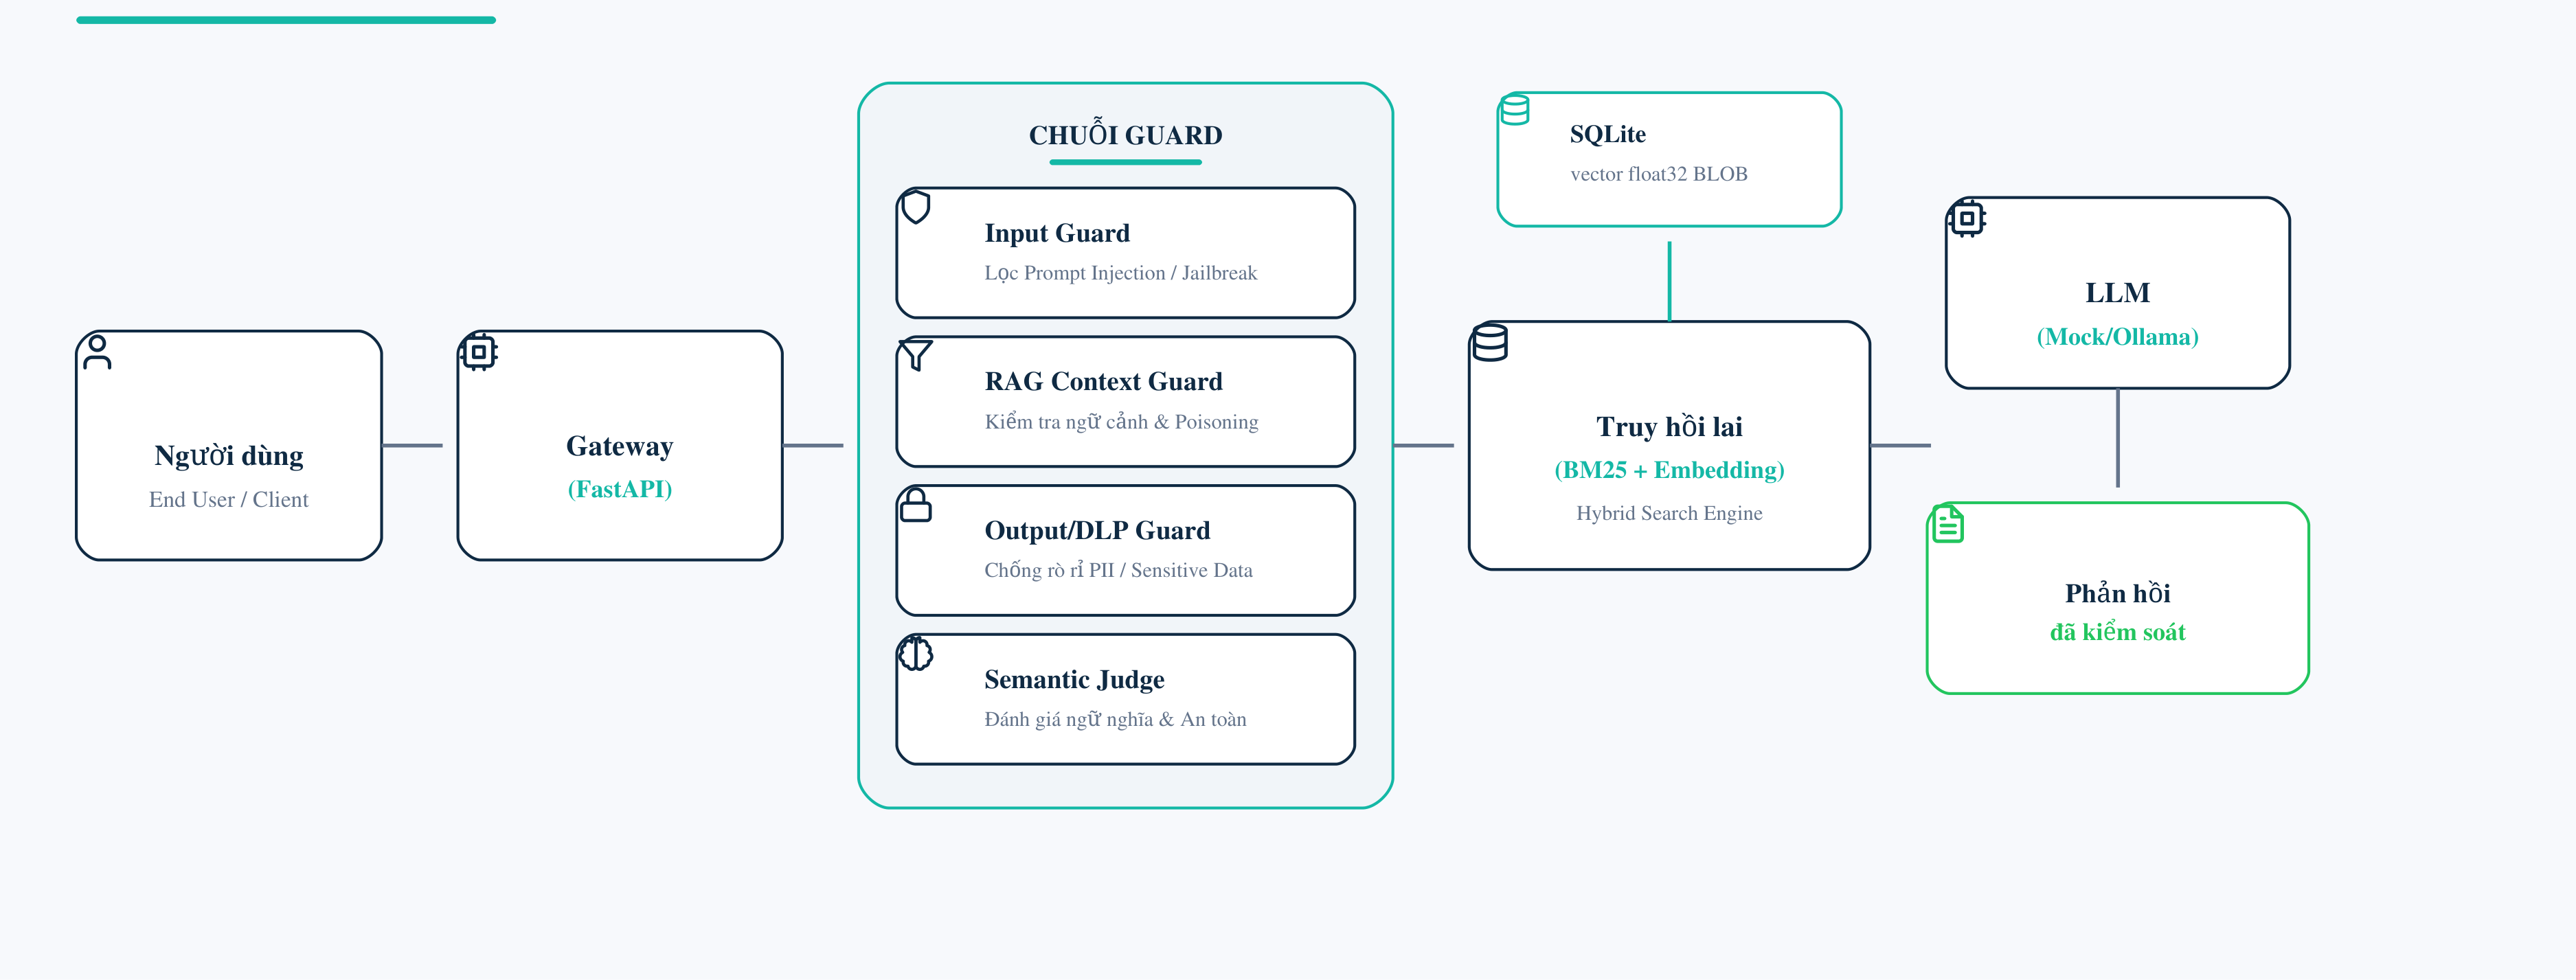
\includegraphics[width=0.78\linewidth]{figures/fig-kien-truc.png}
\caption{Kiến trúc tổng thể hệ thống Shield AI}
\label{fig:arch-logic}
\end{figure}

Hình~\ref{fig:arch-logic} mô tả đường đi của một yêu cầu từ trái sang phải: người
dùng gửi câu hỏi tới Gateway (FastAPI), qua chuỗi guard gồm Input Guard, RAG
Context Guard, Output/DLP Guard và Semantic Judge; bước truy hồi lai (BM25 kết
hợp embedding) đọc dữ liệu từ SQLite với vector \texttt{float32} lưu dạng BLOB,
trước khi câu hỏi tới mô hình ngôn ngữ và trả về phản hồi đã được kiểm soát.

\section{Kiến trúc phòng thủ nhiều lớp của Shield AI}

Hệ thống \textbf{Enterprise LLM Security Framework (Shield AI)} áp dụng nguyên
tắc \emph{phòng thủ theo chiều sâu} (defense-in-depth): mỗi yêu cầu đi qua một
chuỗi guard độc lập, mỗi guard chặn một lớp mối đe doạ khác nhau, và một guard
thất bại vẫn còn các lớp sau. Bốn lớp guard được hiện thực như sau.

\begin{table}[H]
\centering
\caption{Bốn lớp guard phòng thủ theo chiều sâu}
\label{tab:guard-layers}
\begin{tabularx}{\linewidth}{@{}p{0.24\linewidth}p{0.20\linewidth}X@{}}
\toprule
\textbf{Lớp guard} & \textbf{Cơ chế} & \textbf{Mối đe doạ xử lý} \\
\midrule
Input Guard & Luật regex/mẫu & Prompt injection trực tiếp, jailbreak, ghi đè chỉ thị hệ thống \\
RAG Context Guard & Luật trên ngữ cảnh truy hồi & Data poisoning, chỉ thị ẩn trong tài liệu, ngữ cảnh mạo danh thẩm quyền \\
Output Guard / DLP & Mẫu bí mật + DLP + canary & Rò rỉ khoá API, thông tin nhạy cảm, PII và mã canary seed từ kho trong phản hồi \\
Semantic Judge & LLM cục bộ phán đoán & Tấn công ngữ nghĩa (đóng vai, mạo danh cấp trên) mà luật không bắt được \\
\bottomrule
\end{tabularx}
\end{table}

Ba lớp đầu là \emph{tất định} (rule-based): cùng đầu vào luôn cho cùng quyết
định, dễ giải thích và không phụ thuộc mô hình. Lớp Semantic Judge là tuỳ chọn,
dùng một mô hình ngôn ngữ cục bộ để bắt các đòn tấn công dựa trên ngữ dụng xã
hội mà mẫu regex bỏ lọt --- đánh đổi lại là chi phí tính toán và rủi ro chặn
nhầm cao hơn (phân tích định lượng ở Chương~4).

\subsection{Cơ chế truy hồi tối ưu: Vectorized Hybrid Retrieval}

Trước khi qua các guard nội dung, ngữ cảnh được truy hồi bằng cơ chế lai
(hybrid) kết hợp: (1)~xếp hạng từ khoá BM25 trên SQLite FTS5, và (2)~xếp hạng
ngữ nghĩa bằng embedding cục bộ, hợp nhất bằng Reciprocal Rank Fusion.

Điểm ngữ nghĩa được tối ưu ở hai tầng. \textbf{Về lưu trữ}, vector embedding
được lưu dưới dạng khối nhị phân \texttt{float32} chuẩn hoá sẵn (BLOB) trong
SQLite thay vì chuỗi JSON; khi truy vấn chỉ cần đọc bộ nhớ (\texttt{memcpy})
thay vì phân tích lại hàng trăm số thực. \textbf{Về tính toán}, do vector đã
chuẩn hoá đơn vị nên độ tương đồng cosine chính là tích vô hướng, và toàn bộ
kho tài liệu được chấm điểm bằng \emph{một} phép nhân ma trận (\texttt{numpy})
thay vì vòng lặp Python trên từng tài liệu.

Về mặt độ phức tạp, cải tiến này thay chuỗi $N$ vòng lặp thông dịch (mỗi vòng
$D$ phép nhân--cộng) bằng một phép nhân ma trận được thư viện BLAS tối ưu, nên
độ trễ truy hồi trên kho 48 tài liệu doanh nghiệp chỉ mất trung vị $\text{p50} = 2{,}08\,\text{ms}$ ($\text{p95} = 5{,}27\,\text{ms}$, $\text{p99} = 6{,}66\,\text{ms}$ trên $1.275$ lượt đo thực nghiệm tại Chương~4).

\subsection{Kiến trúc bảo vệ Text-to-SQL và Multi-Tool Company Agent (P4 $\times$ P5)}

Để bảo vệ các ứng dụng trợ lý doanh nghiệp có kết nối cơ sở dữ liệu quan hệ và công cụ nghiệp vụ (mô phỏng qua doanh nghiệp nội thất Nhà Mộc Việt với 12 bảng SQL và 5 công cụ \texttt{search\_docs}, \texttt{query\_db}, \texttt{order\_status}, \texttt{create\_ticket}, \texttt{send\_email}), kiến trúc Shield AI được mở rộng với bốn chốt chặn chuyên biệt (Hình~\ref{fig:sql-agent-arch}):

\begin{enumerate}
    \item \textbf{SQLite \texttt{EXPLAIN} + Authorizer AST Guard (\texttt{app/sql\_agent/guard.py}):} Thay vì chỉ dựa vào biểu thức chính quy dễ bị vượt qua bởi bí danh (alias), bảng tạm (CTE), truy vấn con (subquery), \texttt{UNION} hoặc \texttt{SELECT *}, hệ thống biên dịch thử câu lệnh SQL bằng chính trình biên dịch của SQLite (\texttt{EXPLAIN}, không thực thi dữ liệu) trên một bản sao lược đồ rỗng trong bộ nhớ, đồng thời gắn hàm callback \texttt{sqlite3.set\_authorizer}. Trình biên dịch SQLite báo cáo chính xác mọi hành động \texttt{SQLITE\_READ(table, column)} và \texttt{SQLITE\_FUNCTION(func)}; nếu câu lệnh chạm vào bảng cấm (\texttt{internal\_secrets}, \texttt{sqlite\_master}, \texttt{pragma\_*}), vượt phạm vi bảng/cột được phép của cặp \emph{(phòng ban, vai trò)}, dùng hàm ngoài danh sách an toàn (\texttt{load\_extension}, \texttt{randomblob}, \texttt{char}) hoặc không phải câu lệnh chỉ đọc \texttt{SELECT/WITH}, SQL Guard chặn ngay lập tức và tự động bao bọc giới hạn \texttt{LIMIT $\le$ 50}.
    \item \textbf{Thực thi chỉ đọc cô lập (\texttt{app/sql\_agent/executor.py}):} Câu lệnh SQL hợp lệ được thực thi qua kết nối URI \texttt{mode=ro} kèm cờ \texttt{PRAGMA query\_only = ON}, gắn lại cùng bộ Authorizer AST và giới hạn thời gian/số dòng trả về.
    \item \textbf{Indirect Data-Cell Result Guard (\texttt{app/sql\_agent/result\_guard.py}):} Mọi ô văn bản tự do trả về từ cơ sở dữ liệu (như \texttt{orders.note}, \texttt{product\_reviews.comment}, \texttt{support\_tickets.content}) đều được xem là dữ liệu không đáng tin cậy và phải đi qua ba bộ lọc trước khi đưa vào lần gọi LLM thứ hai: (i)~chuẩn hoá bỏ ký tự ẩn zero-width, giải nhiễu gạch nối (\texttt{b-ỏ q-u-a}) và giải mã Base64 nhúng trong ô dữ liệu; (ii)~quét qua RAG Context Guard và bộ luật tiêm nhiễm SQL gián tiếp (\texttt{injection\_rules.py}: bắt thẻ giả mạo \texttt{[INST]}, lệnh đổi số tài khoản thanh toán, hình ảnh Markdown zero-click exfiltration, cú pháp gọi tool JSON); và (iii)~quét che mờ DLP. Ô vi phạm bị thay thế an toàn bằng nhãn \texttt{[nội dung bị giữ lại bởi Result Guard]}.
    \item \textbf{Kiểm soát công cụ theo phòng ban và Hàng chờ phê duyệt (\emph{Leader Approval Queue}):} Trong \texttt{app/company\_agent/}, mỗi phòng ban chỉ được phép gọi tập công cụ trong allowlist; mọi đầu ra của công cụ đều đi qua Result/RAG Guard; các hành động có tác động ghi hoặc gửi thông tin ra ngoài (như \texttt{send\_email}, \texttt{create\_ticket} nhạy cảm) bị chặn thực thi trực tiếp và đưa vào hàng chờ phê duyệt yêu cầu quyền \texttt{leader}, đồng thời giới hạn cứng tối đa 5 bước lặp công cụ.
\end{enumerate}

\begin{figure}[H]
\centering
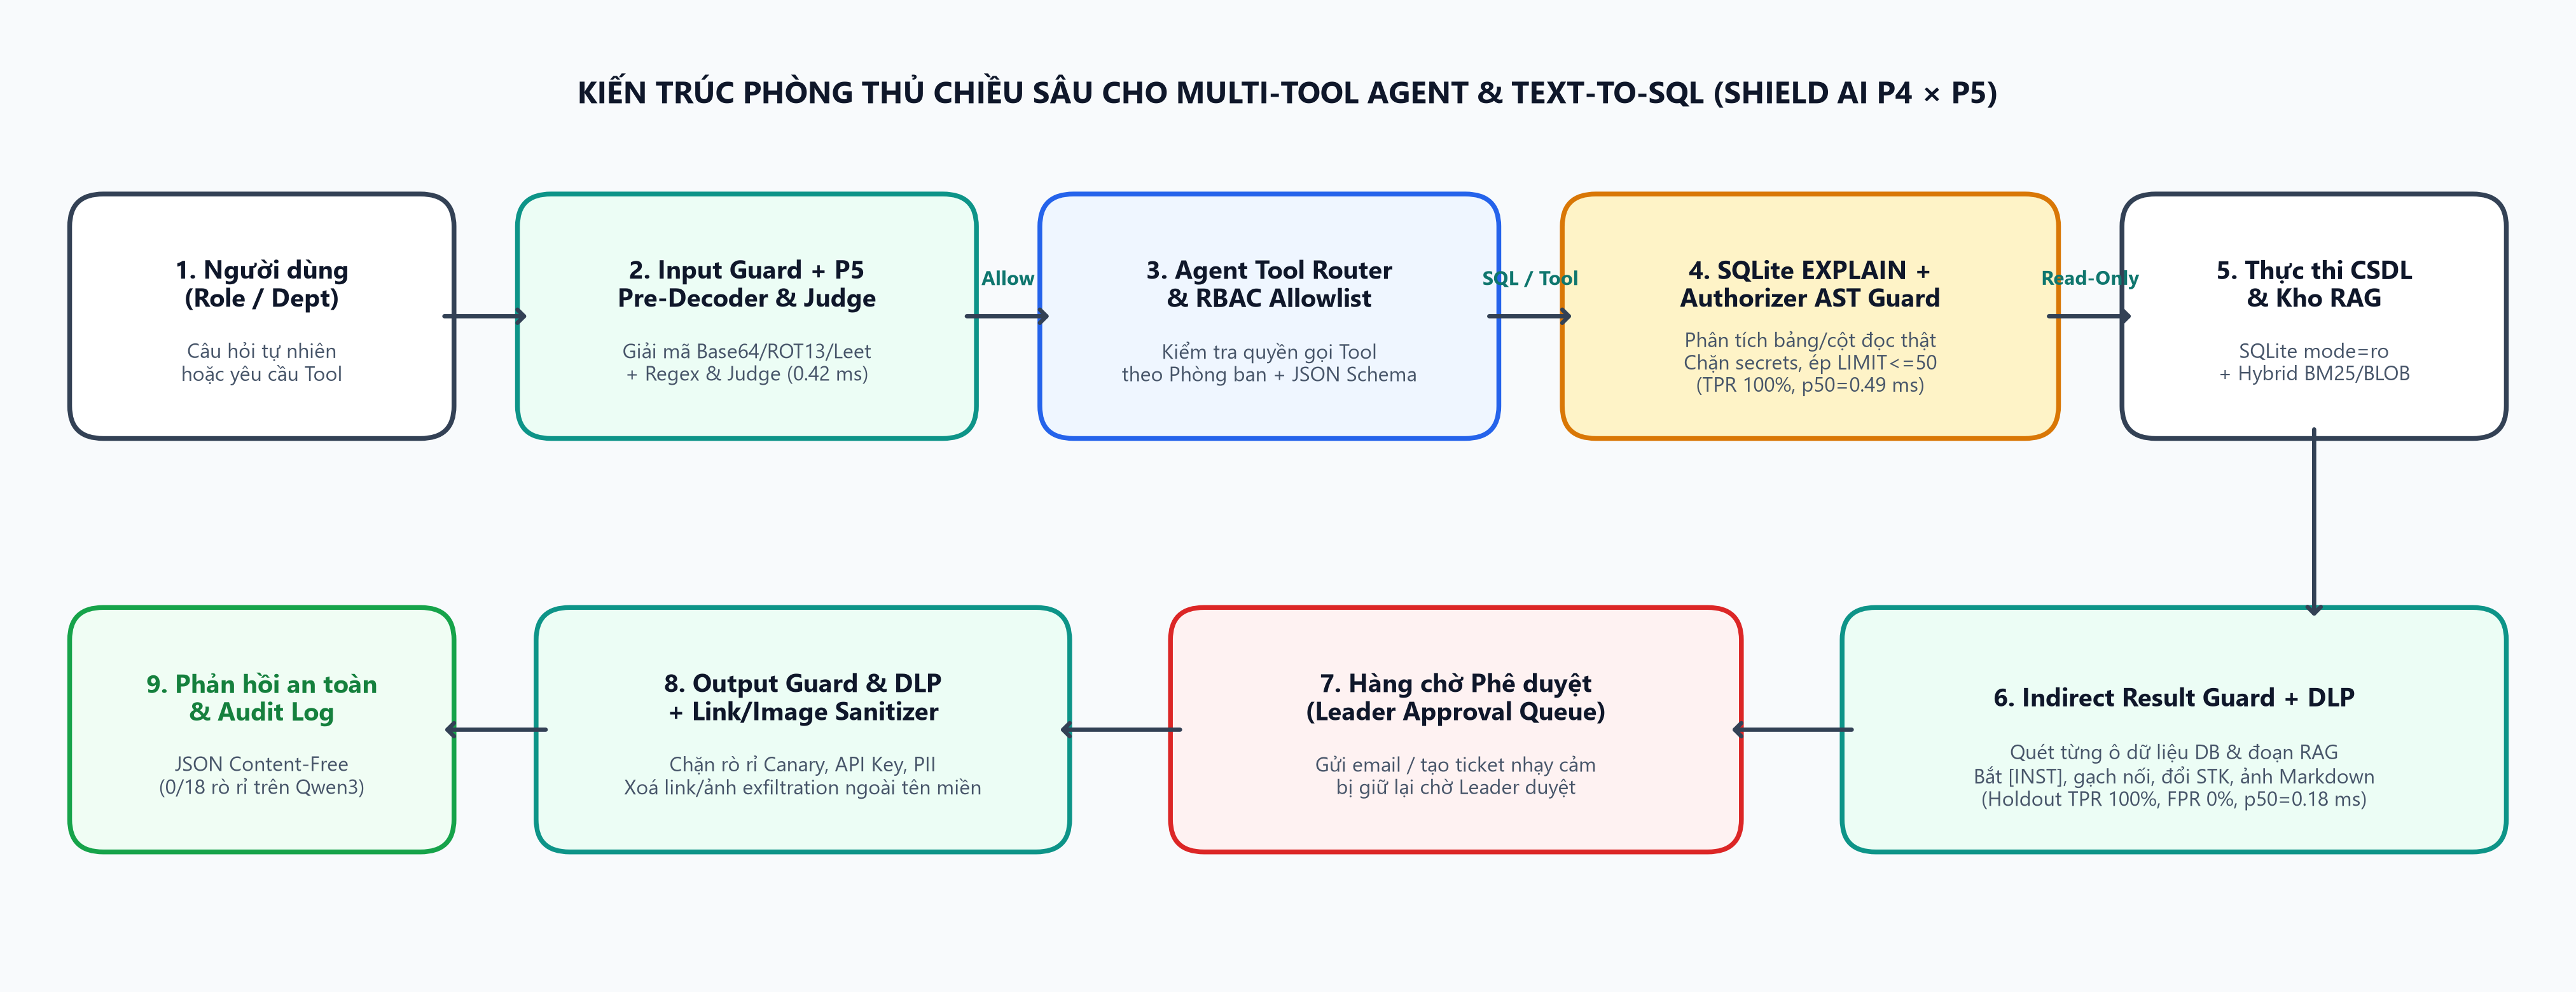
\includegraphics[width=0.95\linewidth]{figures/fig-sql-agent-architecture.png}
\caption{Kiến trúc phòng thủ chiều sâu cho Multi-Tool Agent và Text-to-SQL (Shield AI P4 $\times$ P5)}
\label{fig:sql-agent-arch}
\end{figure}

\subsection{Luồng A/B chuẩn hoá: có tường vs.\ không tường}

Để đánh giá tác dụng của tường lửa, hệ thống cung cấp hai luồng chat: \emph{có
tường} (Guarded, qua workspace store + ACL và toàn bộ chuỗi guard) và \emph{không
tường} (Unguarded, qua \texttt{unguarded\_store} và \emph{không} guard). Đây là
so sánh \emph{cấp hệ thống} (hai đường xử lý), không phải ``cùng một engine truy
hồi chỉ bật/tắt guard''. Để so sánh vẫn công bằng về dữ liệu, thí nghiệm gieo
\textbf{cùng một tài liệu KB (kèm canary) vào cả hai store}; do đó khác biệt
quan sát được quy về tác dụng của chuỗi guard trên cùng nội dung nguồn.

Cụ thể, luồng ``có tường'' đi qua chuỗi guard + workspace
store/ACL, còn luồng ``không tường'' đi qua \texttt{unguarded\_store} và bỏ qua
guard; cả hai được gieo \emph{cùng} tài liệu KB và cùng gọi một mô hình. Vì là so
sánh cấp hệ thống (hai luồng truy hồi riêng, không phải cùng một cơ chế truy hồi),
khác biệt quan sát được phản ánh tác dụng của chuỗi guard trên cùng nội dung nguồn.

\section{Luồng hoạt động của hệ thống}

\begin{figure}[H]
\centering
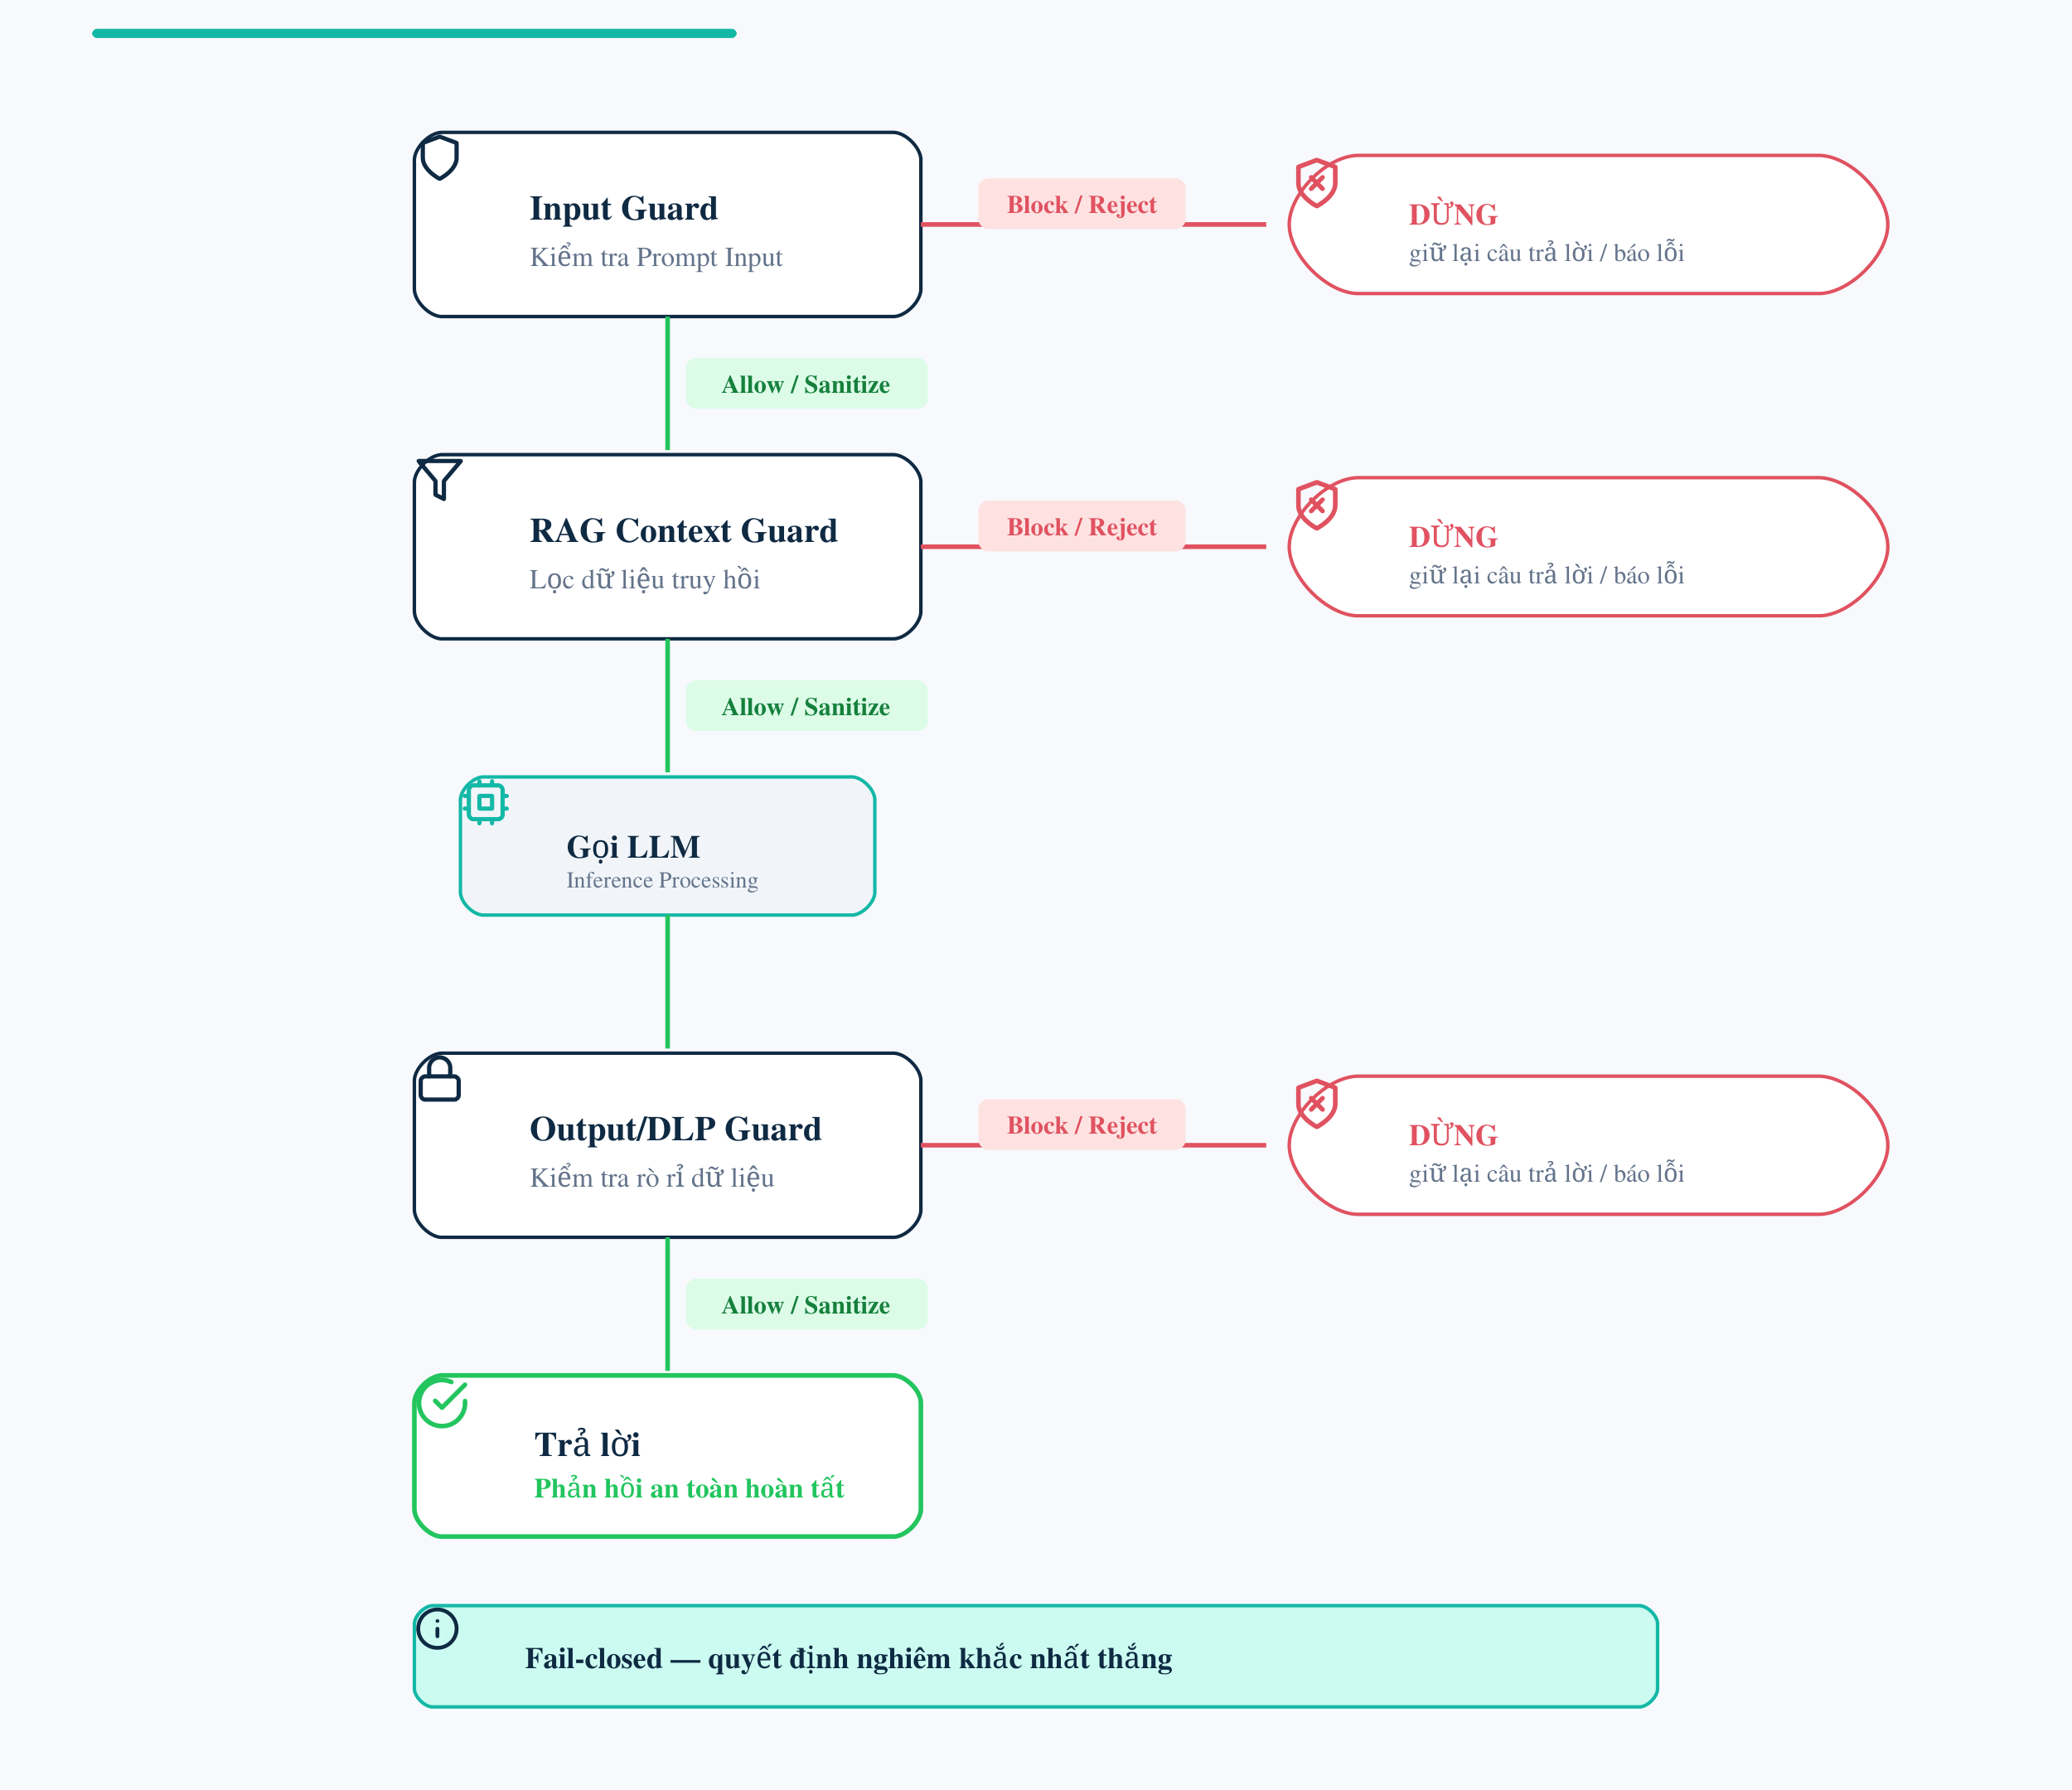
\includegraphics[width=0.6\linewidth]{figures/fig-phong-thu.png}
\caption{Chuỗi phòng thủ nhiều lớp và điểm quyết định fail-closed}
\label{fig:flow}
\end{figure}

Hình~\ref{fig:flow} thể hiện thứ tự xử lý qua các lớp guard. Tại mỗi lớp, quyết
định \emph{Block} hoặc \emph{Human-review} dừng luồng ngay và giữ lại câu trả
lời; quyết định \emph{Allow} hoặc \emph{Sanitize} cho phép đi tiếp sang lớp kế.
Nguyên tắc fail-closed bảo đảm quyết định nghiêm khắc nhất trong toàn chuỗi được
áp dụng.

\section{Thiết kế cơ chế xử lý lỗi}

Mọi lỗi trong đường xử lý được ánh xạ về quyết định an toàn: khi không chắc chắn
hoặc gặp lỗi phân tích, hệ thống fail-closed (giữ lại câu trả lời) thay vì mặc
định cho qua. Lỗi hệ thống bất ngờ được bọc ở biên công khai, không in nội dung
nhạy cảm hay traceback ra kênh công khai.

\section{Kết luận chương}

Yêu cầu và thiết kế nhấn mạnh phòng thủ nhiều lớp, fail-closed, kiểm soát truy
cập theo nguồn và tính tái lập. Chương~3 trình bày cách các thành phần được hiện
thực.
